\documentclass[twoside]{book}

% Packages required by doxygen
\usepackage{calc}
\usepackage{doxygen}
\usepackage{graphicx}
\usepackage[utf8]{inputenc}
\usepackage{makeidx}
\usepackage{multicol}
\usepackage{multirow}
\usepackage{textcomp}
\usepackage[table]{xcolor}

% Font selection
\usepackage[T1]{fontenc}
\usepackage{mathptmx}
\usepackage[scaled=.90]{helvet}
\usepackage{courier}
\usepackage{amssymb}
\usepackage{sectsty}
\renewcommand{\familydefault}{\sfdefault}
\allsectionsfont{%
  \fontseries{bc}\selectfont%
  \color{darkgray}%
}
\renewcommand{\DoxyLabelFont}{%
  \fontseries{bc}\selectfont%
  \color{darkgray}%
}

% Page & text layout
\usepackage{geometry}
\geometry{%
  a4paper,%
  top=2.5cm,%
  bottom=2.5cm,%
  left=2.5cm,%
  right=2.5cm%
}
\tolerance=750
\hfuzz=15pt
\hbadness=750
\setlength{\emergencystretch}{15pt}
\setlength{\parindent}{0cm}
\setlength{\parskip}{0.2cm}
\makeatletter
\renewcommand{\paragraph}{%
  \@startsection{paragraph}{4}{0ex}{-1.0ex}{1.0ex}{%
    \normalfont\normalsize\bfseries\SS@parafont%
  }%
}
\renewcommand{\subparagraph}{%
  \@startsection{subparagraph}{5}{0ex}{-1.0ex}{1.0ex}{%
    \normalfont\normalsize\bfseries\SS@subparafont%
  }%
}
\makeatother

% Headers & footers
\usepackage{fancyhdr}
\pagestyle{fancyplain}
\fancyhead[LE]{\fancyplain{}{\bfseries\thepage}}
\fancyhead[CE]{\fancyplain{}{}}
\fancyhead[RE]{\fancyplain{}{\bfseries\leftmark}}
\fancyhead[LO]{\fancyplain{}{\bfseries\rightmark}}
\fancyhead[CO]{\fancyplain{}{}}
\fancyhead[RO]{\fancyplain{}{\bfseries\thepage}}
\fancyfoot[LE]{\fancyplain{}{}}
\fancyfoot[CE]{\fancyplain{}{}}
\fancyfoot[RE]{\fancyplain{}{\bfseries\scriptsize Generated on Fri Jul 11 2014 16\-:36\-:11 for mac\-D\-S by Doxygen }}
\fancyfoot[LO]{\fancyplain{}{\bfseries\scriptsize Generated on Fri Jul 11 2014 16\-:36\-:11 for mac\-D\-S by Doxygen }}
\fancyfoot[CO]{\fancyplain{}{}}
\fancyfoot[RO]{\fancyplain{}{}}
\renewcommand{\footrulewidth}{0.4pt}
\renewcommand{\chaptermark}[1]{%
  \markboth{#1}{}%
}
\renewcommand{\sectionmark}[1]{%
  \markright{\thesection\ #1}%
}

% Indices & bibliography
\usepackage{natbib}
\usepackage[titles]{tocloft}
\setcounter{tocdepth}{3}
\setcounter{secnumdepth}{5}
\makeindex

% Hyperlinks (required, but should be loaded last)
\usepackage{ifpdf}
\ifpdf
  \usepackage[pdftex,pagebackref=true]{hyperref}
\else
  \usepackage[ps2pdf,pagebackref=true]{hyperref}
\fi
\hypersetup{%
  colorlinks=true,%
  linkcolor=blue,%
  citecolor=blue,%
  unicode%
}

% Custom commands
\newcommand{\clearemptydoublepage}{%
  \newpage{\pagestyle{empty}\cleardoublepage}%
}


%===== C O N T E N T S =====

\begin{document}

% Titlepage & ToC
\hypersetup{pageanchor=false}
\pagenumbering{roman}
\begin{titlepage}
\vspace*{7cm}
\begin{center}%
{\Large mac\-D\-S }\\
\vspace*{1cm}
{\large Generated by Doxygen 1.8.6}\\
\vspace*{0.5cm}
{\small Fri Jul 11 2014 16:36:11}\\
\end{center}
\end{titlepage}
\clearemptydoublepage
\tableofcontents
\clearemptydoublepage
\pagenumbering{arabic}
\hypersetup{pageanchor=true}

%--- Begin generated contents ---
\chapter{Hierarchical Index}
\section{Class Hierarchy}
This inheritance list is sorted roughly, but not completely, alphabetically\-:\begin{DoxyCompactList}
\item $<$N\-S\-Application\-Delegate$>$\begin{DoxyCompactList}
\item \contentsline{section}{M\-D\-App\-Delegate}{\pageref{interface_m_d_app_delegate}}{}
\end{DoxyCompactList}
\item $<$N\-S\-Menu\-Delegate$>$\begin{DoxyCompactList}
\item \contentsline{section}{M\-D\-App\-Delegate}{\pageref{interface_m_d_app_delegate}}{}
\item \contentsline{section}{M\-D\-Zone\-Menu\-Item}{\pageref{interface_m_d_zone_menu_item}}{}
\end{DoxyCompactList}
\item N\-S\-Menu\-Item\begin{DoxyCompactList}
\item \contentsline{section}{M\-D\-Scene\-Menu\-Item}{\pageref{interface_m_d_scene_menu_item}}{}
\begin{DoxyCompactList}
\item \contentsline{section}{M\-D\-Device\-Menu\-Item}{\pageref{interface_m_d_device_menu_item}}{}
\end{DoxyCompactList}
\item \contentsline{section}{M\-D\-Zone\-Menu\-Item}{\pageref{interface_m_d_zone_menu_item}}{}
\end{DoxyCompactList}
\item $<$N\-S\-Net\-Service\-Browser\-Delegate$>$\begin{DoxyCompactList}
\item \contentsline{section}{M\-D\-Main\-Preferences\-View\-Controller}{\pageref{interface_m_d_main_preferences_view_controller}}{}
\end{DoxyCompactList}
\item N\-S\-Object\begin{DoxyCompactList}
\item \contentsline{section}{M\-D\-App\-Delegate}{\pageref{interface_m_d_app_delegate}}{}
\item \contentsline{section}{M\-D\-D\-S\-Helper}{\pageref{interface_m_d_d_s_helper}}{}
\item \contentsline{section}{M\-D\-D\-S\-S\-Manager}{\pageref{interface_m_d_d_s_s_manager}}{}
\item \contentsline{section}{M\-D\-D\-S\-S\-U\-R\-L\-Connection}{\pageref{interface_m_d_d_s_s_u_r_l_connection}}{}
\end{DoxyCompactList}
\item $<$N\-S\-Table\-View\-Data\-Source$>$\begin{DoxyCompactList}
\item \contentsline{section}{M\-D\-Main\-Preferences\-View\-Controller}{\pageref{interface_m_d_main_preferences_view_controller}}{}
\end{DoxyCompactList}
\item $<$N\-S\-Table\-View\-Delegate$>$\begin{DoxyCompactList}
\item \contentsline{section}{M\-D\-Main\-Preferences\-View\-Controller}{\pageref{interface_m_d_main_preferences_view_controller}}{}
\end{DoxyCompactList}
\item $<$N\-S\-Text\-Field\-Delegate$>$\begin{DoxyCompactList}
\item \contentsline{section}{M\-D\-Main\-Preferences\-View\-Controller}{\pageref{interface_m_d_main_preferences_view_controller}}{}
\end{DoxyCompactList}
\item $<$N\-S\-U\-R\-L\-Connection\-Data\-Delegate$>$\begin{DoxyCompactList}
\item \contentsline{section}{M\-D\-D\-S\-S\-Manager}{\pageref{interface_m_d_d_s_s_manager}}{}
\end{DoxyCompactList}
\item $<$N\-S\-U\-R\-L\-Connection\-Delegate$>$\begin{DoxyCompactList}
\item \contentsline{section}{M\-D\-D\-S\-S\-Manager}{\pageref{interface_m_d_d_s_s_manager}}{}
\end{DoxyCompactList}
\item N\-S\-View\-Controller\begin{DoxyCompactList}
\item \contentsline{section}{M\-D\-Main\-Preferences\-View\-Controller}{\pageref{interface_m_d_main_preferences_view_controller}}{}
\end{DoxyCompactList}
\item $<$R\-H\-Preferences\-View\-Controller\-Protocol$>$\begin{DoxyCompactList}
\item \contentsline{section}{M\-D\-Main\-Preferences\-View\-Controller}{\pageref{interface_m_d_main_preferences_view_controller}}{}
\end{DoxyCompactList}
\end{DoxyCompactList}

\chapter{Class Index}
\section{Class List}
Here are the classes, structs, unions and interfaces with brief descriptions\-:\begin{DoxyCompactList}
\item\contentsline{section}{\hyperlink{interface_m_d_app_delegate}{M\-D\-App\-Delegate} }{\pageref{interface_m_d_app_delegate}}{}
\item\contentsline{section}{\hyperlink{interface_m_d_consumption_view}{M\-D\-Consumption\-View} }{\pageref{interface_m_d_consumption_view}}{}
\item\contentsline{section}{\hyperlink{interface_m_d_detail_preferences_view_controller}{M\-D\-Detail\-Preferences\-View\-Controller} }{\pageref{interface_m_d_detail_preferences_view_controller}}{}
\item\contentsline{section}{\hyperlink{interface_m_d_device_menu_item}{M\-D\-Device\-Menu\-Item} }{\pageref{interface_m_d_device_menu_item}}{}
\item\contentsline{section}{\hyperlink{interface_m_d_d_s_helper}{M\-D\-D\-S\-Helper} }{\pageref{interface_m_d_d_s_helper}}{}
\item\contentsline{section}{\hyperlink{interface_m_d_d_s_s_consumption_manager}{M\-D\-D\-S\-S\-Consumption\-Manager} }{\pageref{interface_m_d_d_s_s_consumption_manager}}{}
\item\contentsline{section}{\hyperlink{interface_m_d_d_s_s_manager}{M\-D\-D\-S\-S\-Manager} }{\pageref{interface_m_d_d_s_s_manager}}{}
\item\contentsline{section}{\hyperlink{interface_m_d_d_s_s_u_r_l_connection}{M\-D\-D\-S\-S\-U\-R\-L\-Connection} }{\pageref{interface_m_d_d_s_s_u_r_l_connection}}{}
\item\contentsline{section}{\hyperlink{interface_m_d_main_preferences_view_controller}{M\-D\-Main\-Preferences\-View\-Controller} }{\pageref{interface_m_d_main_preferences_view_controller}}{}
\item\contentsline{section}{\hyperlink{interface_m_d_scene_menu_item}{M\-D\-Scene\-Menu\-Item} }{\pageref{interface_m_d_scene_menu_item}}{}
\item\contentsline{section}{\hyperlink{interface_m_d_zone_menu_item}{M\-D\-Zone\-Menu\-Item} }{\pageref{interface_m_d_zone_menu_item}}{}
\end{DoxyCompactList}

\chapter{Class Documentation}
\hypertarget{interface_m_d_app_delegate}{\section{M\-D\-App\-Delegate Class Reference}
\label{interface_m_d_app_delegate}\index{M\-D\-App\-Delegate@{M\-D\-App\-Delegate}}
}
Inheritance diagram for M\-D\-App\-Delegate\-:\begin{figure}[H]
\begin{center}
\leavevmode
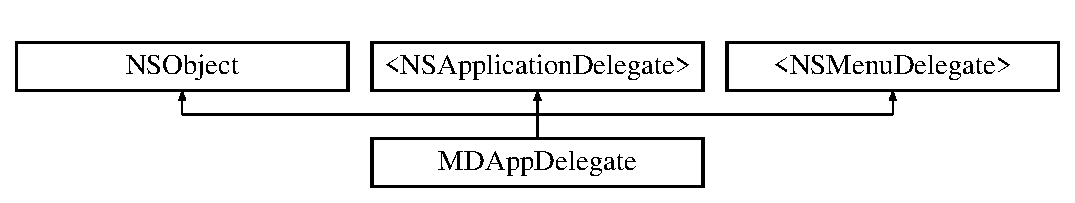
\includegraphics[height=2.000000cm]{interface_m_d_app_delegate}
\end{center}
\end{figure}
\subsection*{Properties}
\begin{DoxyCompactItemize}
\item 
\hypertarget{interface_m_d_app_delegate_a0758151aaf56aadb705303b2715081c8}{I\-B\-Outlet N\-S\-Window $\ast$ {\bfseries window}}\label{interface_m_d_app_delegate_a0758151aaf56aadb705303b2715081c8}

\end{DoxyCompactItemize}


The documentation for this class was generated from the following file\-:\begin{DoxyCompactItemize}
\item 
mac\-D\-S/M\-D\-App\-Delegate.\-h\end{DoxyCompactItemize}

\hypertarget{interface_m_d_consumption_view}{\section{M\-D\-Consumption\-View Class Reference}
\label{interface_m_d_consumption_view}\index{M\-D\-Consumption\-View@{M\-D\-Consumption\-View}}
}
Inheritance diagram for M\-D\-Consumption\-View\-:\begin{figure}[H]
\begin{center}
\leavevmode
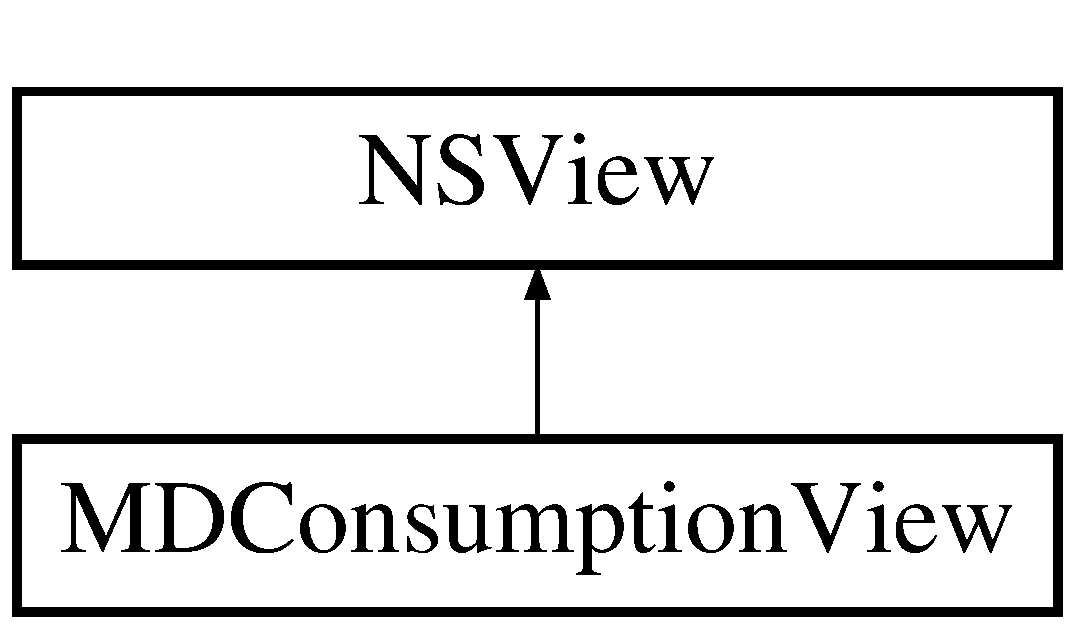
\includegraphics[height=2.000000cm]{interface_m_d_consumption_view}
\end{center}
\end{figure}


The documentation for this class was generated from the following file\-:\begin{DoxyCompactItemize}
\item 
mac\-D\-S/M\-D\-Consumption\-View.\-h\end{DoxyCompactItemize}

\hypertarget{interface_m_d_detail_preferences_view_controller}{\section{M\-D\-Detail\-Preferences\-View\-Controller Class Reference}
\label{interface_m_d_detail_preferences_view_controller}\index{M\-D\-Detail\-Preferences\-View\-Controller@{M\-D\-Detail\-Preferences\-View\-Controller}}
}
Inheritance diagram for M\-D\-Detail\-Preferences\-View\-Controller\-:\begin{figure}[H]
\begin{center}
\leavevmode
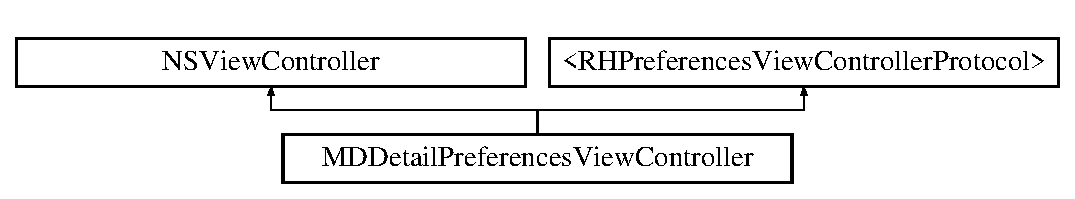
\includegraphics[height=2.000000cm]{interface_m_d_detail_preferences_view_controller}
\end{center}
\end{figure}
\subsection*{Properties}
\begin{DoxyCompactItemize}
\item 
\hypertarget{interface_m_d_detail_preferences_view_controller_a1e1d2f0a61e7275f126f549b807e5e8b}{I\-B\-Outlet N\-S\-Button $\ast$ {\bfseries launch\-At\-Startup\-Button}}\label{interface_m_d_detail_preferences_view_controller_a1e1d2f0a61e7275f126f549b807e5e8b}

\item 
\hypertarget{interface_m_d_detail_preferences_view_controller_aeae32b19a1a02e330a74221fa285a883}{B\-O\-O\-L {\bfseries launch\-At\-Startup}}\label{interface_m_d_detail_preferences_view_controller_aeae32b19a1a02e330a74221fa285a883}

\end{DoxyCompactItemize}


The documentation for this class was generated from the following file\-:\begin{DoxyCompactItemize}
\item 
mac\-D\-S/\-Preferences/M\-D\-Detail\-Preferences\-View\-Controller.\-h\end{DoxyCompactItemize}

\hypertarget{interface_m_d_device_menu_item}{\section{M\-D\-Device\-Menu\-Item Class Reference}
\label{interface_m_d_device_menu_item}\index{M\-D\-Device\-Menu\-Item@{M\-D\-Device\-Menu\-Item}}
}


{\ttfamily \#import $<$M\-D\-Device\-Menu\-Item.\-h$>$}

Inheritance diagram for M\-D\-Device\-Menu\-Item\-:\begin{figure}[H]
\begin{center}
\leavevmode
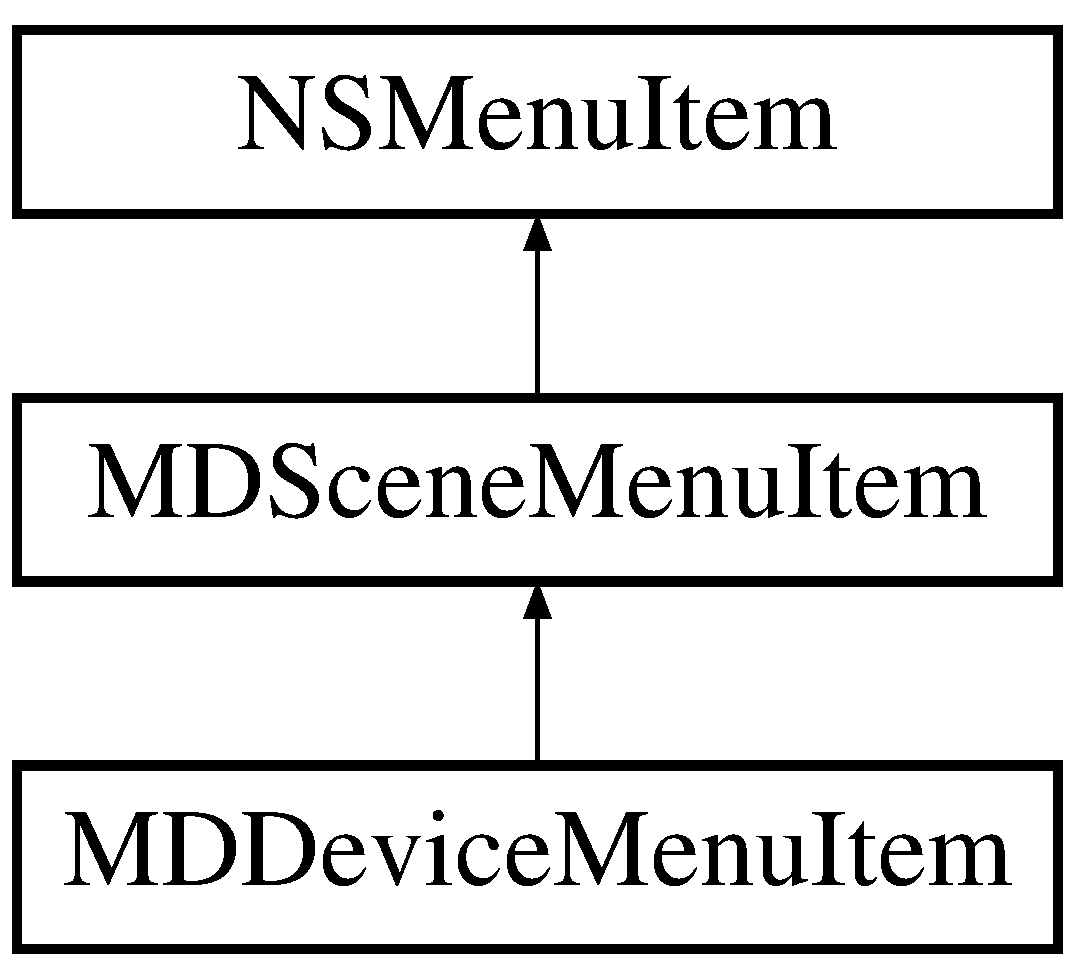
\includegraphics[height=3.000000cm]{interface_m_d_device_menu_item}
\end{center}
\end{figure}
\subsection*{Properties}
\begin{DoxyCompactItemize}
\item 
N\-S\-String $\ast$ \hyperlink{interface_m_d_device_menu_item_aba1a1c831e4cace1935fef25e04a4b27}{dsid}
\item 
\hypertarget{interface_m_d_device_menu_item_a6c6cf5c639107bdcf7abf5d31fe4d553}{B\-O\-O\-L {\bfseries turn\-On\-Off\-Mode}}\label{interface_m_d_device_menu_item_a6c6cf5c639107bdcf7abf5d31fe4d553}

\end{DoxyCompactItemize}


\subsection{Detailed Description}
M\-D\-Zone\-Menu\-Item\-Click\-Type. Class for Device Menu Item 

\subsection{Property Documentation}
\hypertarget{interface_m_d_device_menu_item_aba1a1c831e4cace1935fef25e04a4b27}{\index{M\-D\-Device\-Menu\-Item@{M\-D\-Device\-Menu\-Item}!dsid@{dsid}}
\index{dsid@{dsid}!MDDeviceMenuItem@{M\-D\-Device\-Menu\-Item}}
\subsubsection[{dsid}]{\setlength{\rightskip}{0pt plus 5cm}-\/ (N\-S\-String$\ast$) dsid\hspace{0.3cm}{\ttfamily [read]}, {\ttfamily [write]}, {\ttfamily [atomic]}, {\ttfamily [strong]}}}\label{interface_m_d_device_menu_item_aba1a1c831e4cace1935fef25e04a4b27}
the related dsid for this device 

The documentation for this class was generated from the following file\-:\begin{DoxyCompactItemize}
\item 
D\-S\-Menu/\-Menu/M\-D\-Device\-Menu\-Item.\-h\end{DoxyCompactItemize}

\hypertarget{interface_m_d_d_s_helper}{\section{M\-D\-D\-S\-Helper Class Reference}
\label{interface_m_d_d_s_helper}\index{M\-D\-D\-S\-Helper@{M\-D\-D\-S\-Helper}}
}
Inheritance diagram for M\-D\-D\-S\-Helper\-:\begin{figure}[H]
\begin{center}
\leavevmode
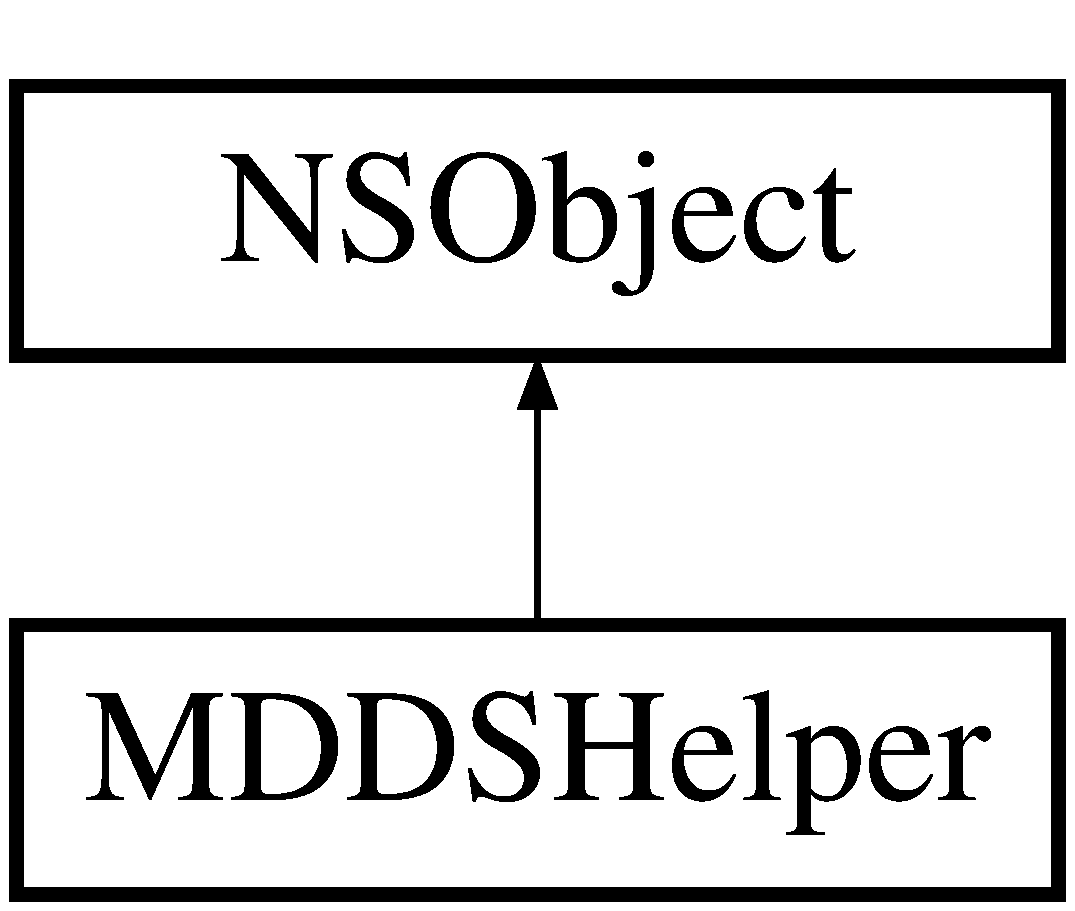
\includegraphics[height=2.000000cm]{interface_m_d_d_s_helper}
\end{center}
\end{figure}
\subsection*{Class Methods}
\begin{DoxyCompactItemize}
\item 
\hypertarget{interface_m_d_d_s_helper_a3f32213841f6409bca57bb0aa3d4d5c1}{(N\-S\-Image $\ast$) + {\bfseries icon\-For\-Device\-:}}\label{interface_m_d_d_s_helper_a3f32213841f6409bca57bb0aa3d4d5c1}

\item 
\hypertarget{interface_m_d_d_s_helper_ad7a3c10995dc96733a6ac86b30de6f2d}{(N\-S\-String $\ast$) + {\bfseries custom\-Scene\-Name\-For\-Scene\-:from\-J\-S\-O\-N\-:}}\label{interface_m_d_d_s_helper_ad7a3c10995dc96733a6ac86b30de6f2d}

\item 
\hypertarget{interface_m_d_d_s_helper_a81f16075bd0ff53c55472f89ed35f994}{(B\-O\-O\-L) + {\bfseries device\-:has\-Group\-:}}\label{interface_m_d_d_s_helper_a81f16075bd0ff53c55472f89ed35f994}

\item 
\hypertarget{interface_m_d_d_s_helper_aaea456daff4bdf1ce9f46850579d172e}{(B\-O\-O\-L) + {\bfseries has\-Group\-:in\-Zone\-:}}\label{interface_m_d_d_s_helper_aaea456daff4bdf1ce9f46850579d172e}

\end{DoxyCompactItemize}


The documentation for this class was generated from the following file\-:\begin{DoxyCompactItemize}
\item 
D\-S\-Menu/M\-D\-D\-S\-Helper.\-h\end{DoxyCompactItemize}

\hypertarget{interface_m_d_d_s_s_consumption_manager}{\section{M\-D\-D\-S\-S\-Consumption\-Manager Class Reference}
\label{interface_m_d_d_s_s_consumption_manager}\index{M\-D\-D\-S\-S\-Consumption\-Manager@{M\-D\-D\-S\-S\-Consumption\-Manager}}
}


{\ttfamily \#import $<$M\-D\-D\-S\-S\-Consumption\-Manager.\-h$>$}

Inheritance diagram for M\-D\-D\-S\-S\-Consumption\-Manager\-:\begin{figure}[H]
\begin{center}
\leavevmode
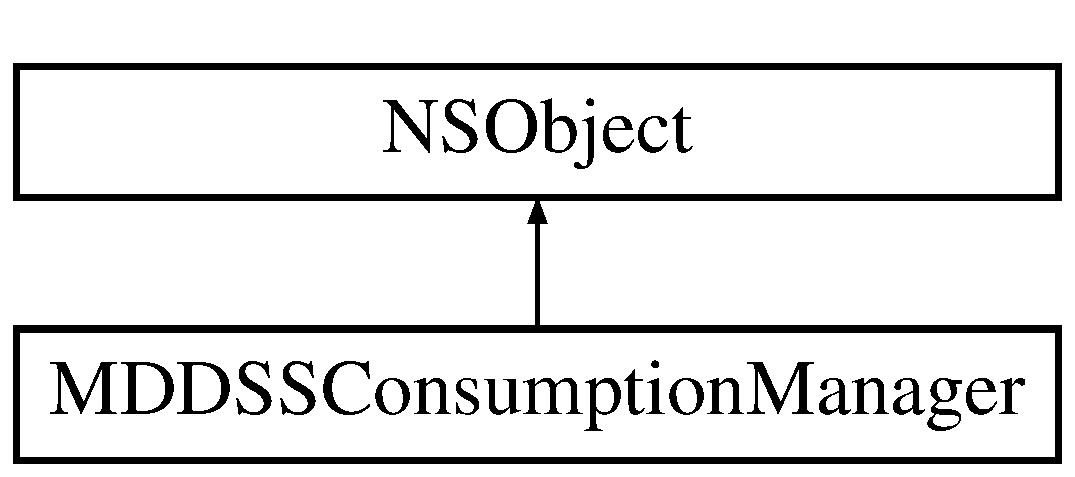
\includegraphics[height=2.000000cm]{interface_m_d_d_s_s_consumption_manager}
\end{center}
\end{figure}
\subsection*{Instance Methods}
\begin{DoxyCompactItemize}
\item 
(void) -\/ \hyperlink{interface_m_d_d_s_s_consumption_manager_aacfaedb3584a13fbeda5f2cf67223ce8}{start\-Polling\-Latest\-:}
\item 
(void) -\/ \hyperlink{interface_m_d_d_s_s_consumption_manager_a9a21d799de7fc9069558a53c73cdfb9c}{start\-Polling\-History\-:}
\item 
(void) -\/ \hyperlink{interface_m_d_d_s_s_consumption_manager_af253ad6e5f08008ceec0a247a27b2526}{stop\-Polling\-Latest}
\item 
(void) -\/ \hyperlink{interface_m_d_d_s_s_consumption_manager_a5c9bf787dd26bf05d1185cf06412ba32}{stop\-Polling\-History}
\item 
(N\-S\-String $\ast$) -\/ \hyperlink{interface_m_d_d_s_s_consumption_manager_a4347a6f14215e842e5629072c1a883c4}{d\-S\-M\-Name\-From\-I\-D\-:}
\item 
(void) -\/ \hyperlink{interface_m_d_d_s_s_consumption_manager_ac4d5086c7cf8ce63e8e3996ba5e841ea}{draw\-History\-On\-Context\-:size\-:}
\end{DoxyCompactItemize}
\subsection*{Class Methods}
\begin{DoxyCompactItemize}
\item 
(\hyperlink{interface_m_d_d_s_s_consumption_manager}{M\-D\-D\-S\-S\-Consumption\-Manager} $\ast$) + \hyperlink{interface_m_d_d_s_s_consumption_manager_ac7a7890115eff0ddaf1e4022d474f4bc}{default\-Manager}
\end{DoxyCompactItemize}
\subsection*{Properties}
\begin{DoxyCompactItemize}
\item 
\hypertarget{interface_m_d_d_s_s_consumption_manager_a911f8a05a99ca741b5e36c59bab6f85f}{void($^\wedge$ {\bfseries callback\-Latest} )(N\-S\-Array $\ast$, N\-S\-Error $\ast$)}\label{interface_m_d_d_s_s_consumption_manager_a911f8a05a99ca741b5e36c59bab6f85f}

\item 
\hypertarget{interface_m_d_d_s_s_consumption_manager_a710c4c8abe3ecfb0555ae66cd7c0d938}{void($^\wedge$ {\bfseries callback\-History} )(N\-S\-Dictionary $\ast$, N\-S\-Array $\ast$)}\label{interface_m_d_d_s_s_consumption_manager_a710c4c8abe3ecfb0555ae66cd7c0d938}

\end{DoxyCompactItemize}


\subsection{Detailed Description}
M\-D\-D\-S\-S\-Enegry\-Manager. This class handles asynchronous polling of consumption data. 

\subsection{Method Documentation}
\hypertarget{interface_m_d_d_s_s_consumption_manager_ac7a7890115eff0ddaf1e4022d474f4bc}{\index{M\-D\-D\-S\-S\-Consumption\-Manager@{M\-D\-D\-S\-S\-Consumption\-Manager}!default\-Manager@{default\-Manager}}
\index{default\-Manager@{default\-Manager}!MDDSSConsumptionManager@{M\-D\-D\-S\-S\-Consumption\-Manager}}
\subsubsection[{default\-Manager}]{\setlength{\rightskip}{0pt plus 5cm}+ ({\bf M\-D\-D\-S\-S\-Consumption\-Manager} $\ast$) default\-Manager 
\begin{DoxyParamCaption}
{}
\end{DoxyParamCaption}
}}\label{interface_m_d_d_s_s_consumption_manager_ac7a7890115eff0ddaf1e4022d474f4bc}
singleton \hypertarget{interface_m_d_d_s_s_consumption_manager_ac4d5086c7cf8ce63e8e3996ba5e841ea}{\index{M\-D\-D\-S\-S\-Consumption\-Manager@{M\-D\-D\-S\-S\-Consumption\-Manager}!draw\-History\-On\-Context\-:size\-:@{draw\-History\-On\-Context\-:size\-:}}
\index{draw\-History\-On\-Context\-:size\-:@{draw\-History\-On\-Context\-:size\-:}!MDDSSConsumptionManager@{M\-D\-D\-S\-S\-Consumption\-Manager}}
\subsubsection[{draw\-History\-On\-Context\-:size\-:}]{\setlength{\rightskip}{0pt plus 5cm}-\/ (void) draw\-History\-On\-Context\-: 
\begin{DoxyParamCaption}
\item[{(C\-G\-Context\-Ref)}]{image\-Context}
\item[{size:(C\-G\-Size)}]{size}
\end{DoxyParamCaption}
}}\label{interface_m_d_d_s_s_consumption_manager_ac4d5086c7cf8ce63e8e3996ba5e841ea}
draw the history on a context \hypertarget{interface_m_d_d_s_s_consumption_manager_a4347a6f14215e842e5629072c1a883c4}{\index{M\-D\-D\-S\-S\-Consumption\-Manager@{M\-D\-D\-S\-S\-Consumption\-Manager}!d\-S\-M\-Name\-From\-I\-D\-:@{d\-S\-M\-Name\-From\-I\-D\-:}}
\index{d\-S\-M\-Name\-From\-I\-D\-:@{d\-S\-M\-Name\-From\-I\-D\-:}!MDDSSConsumptionManager@{M\-D\-D\-S\-S\-Consumption\-Manager}}
\subsubsection[{d\-S\-M\-Name\-From\-I\-D\-:}]{\setlength{\rightskip}{0pt plus 5cm}-\/ (N\-S\-String $\ast$) d\-S\-M\-Name\-From\-I\-D\-: 
\begin{DoxyParamCaption}
\item[{(N\-S\-String $\ast$)}]{dsid}
\end{DoxyParamCaption}
}}\label{interface_m_d_d_s_s_consumption_manager_a4347a6f14215e842e5629072c1a883c4}
Helper for getting d\-S\-M name by dsid out of the cache \hypertarget{interface_m_d_d_s_s_consumption_manager_a9a21d799de7fc9069558a53c73cdfb9c}{\index{M\-D\-D\-S\-S\-Consumption\-Manager@{M\-D\-D\-S\-S\-Consumption\-Manager}!start\-Polling\-History\-:@{start\-Polling\-History\-:}}
\index{start\-Polling\-History\-:@{start\-Polling\-History\-:}!MDDSSConsumptionManager@{M\-D\-D\-S\-S\-Consumption\-Manager}}
\subsubsection[{start\-Polling\-History\-:}]{\setlength{\rightskip}{0pt plus 5cm}-\/ (void) start\-Polling\-History\-: 
\begin{DoxyParamCaption}
\item[{(N\-S\-Integer)}]{intervall\-In\-Seconds}
\end{DoxyParamCaption}
}}\label{interface_m_d_d_s_s_consumption_manager_a9a21d799de7fc9069558a53c73cdfb9c}
start repeatedly polling the dss to get the history consumption values of all d\-S\-Ms \hypertarget{interface_m_d_d_s_s_consumption_manager_aacfaedb3584a13fbeda5f2cf67223ce8}{\index{M\-D\-D\-S\-S\-Consumption\-Manager@{M\-D\-D\-S\-S\-Consumption\-Manager}!start\-Polling\-Latest\-:@{start\-Polling\-Latest\-:}}
\index{start\-Polling\-Latest\-:@{start\-Polling\-Latest\-:}!MDDSSConsumptionManager@{M\-D\-D\-S\-S\-Consumption\-Manager}}
\subsubsection[{start\-Polling\-Latest\-:}]{\setlength{\rightskip}{0pt plus 5cm}-\/ (void) start\-Polling\-Latest\-: 
\begin{DoxyParamCaption}
\item[{(N\-S\-Integer)}]{intervall\-In\-Seconds}
\end{DoxyParamCaption}
}}\label{interface_m_d_d_s_s_consumption_manager_aacfaedb3584a13fbeda5f2cf67223ce8}
start repeatedly polling the dss to get latest consumption values of all d\-S\-Ms \hypertarget{interface_m_d_d_s_s_consumption_manager_a5c9bf787dd26bf05d1185cf06412ba32}{\index{M\-D\-D\-S\-S\-Consumption\-Manager@{M\-D\-D\-S\-S\-Consumption\-Manager}!stop\-Polling\-History@{stop\-Polling\-History}}
\index{stop\-Polling\-History@{stop\-Polling\-History}!MDDSSConsumptionManager@{M\-D\-D\-S\-S\-Consumption\-Manager}}
\subsubsection[{stop\-Polling\-History}]{\setlength{\rightskip}{0pt plus 5cm}-\/ (void) stop\-Polling\-History 
\begin{DoxyParamCaption}
{}
\end{DoxyParamCaption}
}}\label{interface_m_d_d_s_s_consumption_manager_a5c9bf787dd26bf05d1185cf06412ba32}
stop polling history \hypertarget{interface_m_d_d_s_s_consumption_manager_af253ad6e5f08008ceec0a247a27b2526}{\index{M\-D\-D\-S\-S\-Consumption\-Manager@{M\-D\-D\-S\-S\-Consumption\-Manager}!stop\-Polling\-Latest@{stop\-Polling\-Latest}}
\index{stop\-Polling\-Latest@{stop\-Polling\-Latest}!MDDSSConsumptionManager@{M\-D\-D\-S\-S\-Consumption\-Manager}}
\subsubsection[{stop\-Polling\-Latest}]{\setlength{\rightskip}{0pt plus 5cm}-\/ (void) stop\-Polling\-Latest 
\begin{DoxyParamCaption}
{}
\end{DoxyParamCaption}
}}\label{interface_m_d_d_s_s_consumption_manager_af253ad6e5f08008ceec0a247a27b2526}
stop polling latest data 

The documentation for this class was generated from the following file\-:\begin{DoxyCompactItemize}
\item 
mac\-D\-S/\-M\-D\-D\-S\-S\-Manager/M\-D\-D\-S\-S\-Consumption\-Manager.\-h\end{DoxyCompactItemize}

\hypertarget{interface_m_d_d_s_s_manager}{\section{M\-D\-D\-S\-S\-Manager Class Reference}
\label{interface_m_d_d_s_s_manager}\index{M\-D\-D\-S\-S\-Manager@{M\-D\-D\-S\-S\-Manager}}
}


{\ttfamily \#import $<$M\-D\-D\-S\-S\-Manager.\-h$>$}

Inheritance diagram for M\-D\-D\-S\-S\-Manager\-:\begin{figure}[H]
\begin{center}
\leavevmode
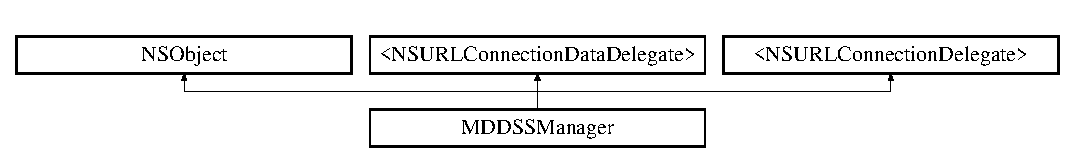
\includegraphics[height=1.744548cm]{interface_m_d_d_s_s_manager}
\end{center}
\end{figure}
\subsection*{Instance Methods}
\begin{DoxyCompactItemize}
\item 
(void) -\/ \hyperlink{interface_m_d_d_s_s_manager_a7fc82977a968af77139dfd04e407a242}{set\-And\-Persist\-Host\-:}
\item 
(void) -\/ \hyperlink{interface_m_d_d_s_s_manager_aa343aa36fdf36c13752a1f0542f04b42}{check\-Host\-:callback\-:}
\item 
(void) -\/ \hyperlink{interface_m_d_d_s_s_manager_a74358d521e85fc2a1a04f15bd8b3954e}{get\-Version\-:}
\item 
(void) -\/ \hyperlink{interface_m_d_d_s_s_manager_a372f9b7faa41788df9a0051cbb3001d6}{get\-Structure\-:}
\item 
(void) -\/ \hyperlink{interface_m_d_d_s_s_manager_af23ff713c6f0860924c0fa55cff11acd}{get\-Structure\-With\-Custom\-Scene\-Names\-:}
\item 
(void) -\/ \hyperlink{interface_m_d_d_s_s_manager_a132057831e843d4888c44f7147ad28a1}{request\-Application\-Token\-:}
\item 
(void) -\/ \hyperlink{interface_m_d_d_s_s_manager_a5380dc94b95172a6131901f23a73bd7d}{call\-Scene\-:zone\-Id\-:group\-I\-D\-:callback\-:}
\item 
(void) -\/ \hyperlink{interface_m_d_d_s_s_manager_a33e9c999b7b7547d42c4102097102ee8}{call\-Scene\-:device\-Id\-:callback\-:}
\item 
(N\-S\-Array $\ast$) -\/ \hyperlink{interface_m_d_d_s_s_manager_a879391644298f08b9dd399d69dc5b137}{custom\-Scene\-Names\-For\-Group\-:in\-Zone\-:}
\item 
(void) -\/ \hyperlink{interface_m_d_d_s_s_manager_afd4b532e4a25c628ff150eb2199515da}{reset\-To\-Defaults}
\item 
\hypertarget{interface_m_d_d_s_s_manager_aafaa7083382f6e128205d821f6adeacd}{(void) -\/ {\bfseries get\-Sensor\-Values\-:}}\label{interface_m_d_d_s_s_manager_aafaa7083382f6e128205d821f6adeacd}

\item 
\hypertarget{interface_m_d_d_s_s_manager_a88e46a8084e45775c057a1849c046ed5}{(void) -\/ {\bfseries set\-Sensor\-Table}}\label{interface_m_d_d_s_s_manager_a88e46a8084e45775c057a1849c046ed5}

\item 
\hypertarget{interface_m_d_d_s_s_manager_a13132214fe9bb3b269804c68f880707f}{(void) -\/ {\bfseries turn\-On\-Device\-Id\-:callback\-:}}\label{interface_m_d_d_s_s_manager_a13132214fe9bb3b269804c68f880707f}

\item 
\hypertarget{interface_m_d_d_s_s_manager_ac96629f2d573ee6acb469892c649533c}{(void) -\/ {\bfseries turn\-Off\-Device\-Id\-:callback\-:}}\label{interface_m_d_d_s_s_manager_ac96629f2d573ee6acb469892c649533c}

\item 
\hypertarget{interface_m_d_d_s_s_manager_a28b119a86c4ce5baaf5900800b404f74}{(void) -\/ {\bfseries get\-Consumption\-Levels\-Latest\-:}}\label{interface_m_d_d_s_s_manager_a28b119a86c4ce5baaf5900800b404f74}

\item 
\hypertarget{interface_m_d_d_s_s_manager_a84579d1873d6ca19a693c972296ebdcc}{(void) -\/ {\bfseries get\-Consumption\-Levels\-D\-S\-I\-D\-:callback\-:}}\label{interface_m_d_d_s_s_manager_a84579d1873d6ca19a693c972296ebdcc}

\item 
\hypertarget{interface_m_d_d_s_s_manager_ae616b77a6cd640f66217ea2aa70bc8a1}{(void) -\/ {\bfseries get\-Circuits\-:}}\label{interface_m_d_d_s_s_manager_ae616b77a6cd640f66217ea2aa70bc8a1}

\end{DoxyCompactItemize}
\subsection*{Class Methods}
\begin{DoxyCompactItemize}
\item 
(\hyperlink{interface_m_d_d_s_s_manager}{M\-D\-D\-S\-S\-Manager} $\ast$) + \hyperlink{interface_m_d_d_s_s_manager_af0359d38979df1d414575dfb7aa6b537}{default\-Manager}
\end{DoxyCompactItemize}
\subsection*{Properties}
\begin{DoxyCompactItemize}
\item 
N\-S\-String $\ast$ \hyperlink{interface_m_d_d_s_s_manager_a27147ce2bf5c9186c96503588983c047}{app\-Name}
\item 
N\-S\-String $\ast$ \hyperlink{interface_m_d_d_s_s_manager_a55aa29ea7dc235519473b2e4ea44c48c}{host}
\item 
\hypertarget{interface_m_d_d_s_s_manager_a2ff1c553be5c3e501021e1d13afdd634}{N\-S\-String $\ast$ {\bfseries port}}\label{interface_m_d_d_s_s_manager_a2ff1c553be5c3e501021e1d13afdd634}

\item 
B\-O\-O\-L \hyperlink{interface_m_d_d_s_s_manager_a25dada9b29593dcd220590d8fdabc58a}{has\-Application\-Token}
\item 
\hypertarget{interface_m_d_d_s_s_manager_a9c7d4d54ae3f3d0a182543929310549d}{N\-S\-String $\ast$ {\bfseries application\-Token}}\label{interface_m_d_d_s_s_manager_a9c7d4d54ae3f3d0a182543929310549d}

\item 
N\-S\-String $\ast$ \hyperlink{interface_m_d_d_s_s_manager_a49c80f7f7f2042658136095fe9f6928f}{d\-S\-S\-Version\-String}
\item 
B\-O\-O\-L \hyperlink{interface_m_d_d_s_s_manager_a4851a2746d573ed0bceddef07fd520f7}{use\-I\-P\-Address}
\end{DoxyCompactItemize}


\subsection{Detailed Description}
D\-S\-S\-Manager class. Layer between App and I\-Net Connection 

\subsection{Method Documentation}
\hypertarget{interface_m_d_d_s_s_manager_a33e9c999b7b7547d42c4102097102ee8}{\index{M\-D\-D\-S\-S\-Manager@{M\-D\-D\-S\-S\-Manager}!call\-Scene\-:device\-Id\-:callback\-:@{call\-Scene\-:device\-Id\-:callback\-:}}
\index{call\-Scene\-:device\-Id\-:callback\-:@{call\-Scene\-:device\-Id\-:callback\-:}!MDDSSManager@{M\-D\-D\-S\-S\-Manager}}
\subsubsection[{call\-Scene\-:device\-Id\-:callback\-:}]{\setlength{\rightskip}{0pt plus 5cm}-\/ (void) call\-Scene\-: 
\begin{DoxyParamCaption}
\item[{(N\-S\-String $\ast$)}]{scene\-Number}
\item[{deviceId:(N\-S\-String $\ast$)}]{device\-Id}
\item[{callback:(void($^\wedge$)(N\-S\-Dictionary $\ast$, N\-S\-Error $\ast$))}]{callback}
\end{DoxyParamCaption}
}}\label{interface_m_d_d_s_s_manager_a33e9c999b7b7547d42c4102097102ee8}
call a scene on a device \hypertarget{interface_m_d_d_s_s_manager_a5380dc94b95172a6131901f23a73bd7d}{\index{M\-D\-D\-S\-S\-Manager@{M\-D\-D\-S\-S\-Manager}!call\-Scene\-:zone\-Id\-:group\-I\-D\-:callback\-:@{call\-Scene\-:zone\-Id\-:group\-I\-D\-:callback\-:}}
\index{call\-Scene\-:zone\-Id\-:group\-I\-D\-:callback\-:@{call\-Scene\-:zone\-Id\-:group\-I\-D\-:callback\-:}!MDDSSManager@{M\-D\-D\-S\-S\-Manager}}
\subsubsection[{call\-Scene\-:zone\-Id\-:group\-I\-D\-:callback\-:}]{\setlength{\rightskip}{0pt plus 5cm}-\/ (void) call\-Scene\-: 
\begin{DoxyParamCaption}
\item[{(N\-S\-String $\ast$)}]{scene\-Number}
\item[{zoneId:(N\-S\-String $\ast$)}]{zone\-Id}
\item[{groupID:(N\-S\-String $\ast$)}]{group\-I\-D}
\item[{callback:(void($^\wedge$)(N\-S\-Dictionary $\ast$, N\-S\-Error $\ast$))}]{callback}
\end{DoxyParamCaption}
}}\label{interface_m_d_d_s_s_manager_a5380dc94b95172a6131901f23a73bd7d}
call a scene on a zone \hypertarget{interface_m_d_d_s_s_manager_aa343aa36fdf36c13752a1f0542f04b42}{\index{M\-D\-D\-S\-S\-Manager@{M\-D\-D\-S\-S\-Manager}!check\-Host\-:callback\-:@{check\-Host\-:callback\-:}}
\index{check\-Host\-:callback\-:@{check\-Host\-:callback\-:}!MDDSSManager@{M\-D\-D\-S\-S\-Manager}}
\subsubsection[{check\-Host\-:callback\-:}]{\setlength{\rightskip}{0pt plus 5cm}-\/ (void) check\-Host\-: 
\begin{DoxyParamCaption}
\item[{(N\-S\-String $\ast$)}]{host}
\item[{callback:(void($^\wedge$)(B\-O\-O\-L))}]{handler}
\end{DoxyParamCaption}
}}\label{interface_m_d_d_s_s_manager_aa343aa36fdf36c13752a1f0542f04b42}
check if behind a host is a d\-S\-S \hypertarget{interface_m_d_d_s_s_manager_a879391644298f08b9dd399d69dc5b137}{\index{M\-D\-D\-S\-S\-Manager@{M\-D\-D\-S\-S\-Manager}!custom\-Scene\-Names\-For\-Group\-:in\-Zone\-:@{custom\-Scene\-Names\-For\-Group\-:in\-Zone\-:}}
\index{custom\-Scene\-Names\-For\-Group\-:in\-Zone\-:@{custom\-Scene\-Names\-For\-Group\-:in\-Zone\-:}!MDDSSManager@{M\-D\-D\-S\-S\-Manager}}
\subsubsection[{custom\-Scene\-Names\-For\-Group\-:in\-Zone\-:}]{\setlength{\rightskip}{0pt plus 5cm}-\/ (N\-S\-Array $\ast$) custom\-Scene\-Names\-For\-Group\-: 
\begin{DoxyParamCaption}
\item[{(int)}]{for\-Group}
\item[{inZone:(int)}]{for\-Zone\-Id}
\end{DoxyParamCaption}
}}\label{interface_m_d_d_s_s_manager_a879391644298f08b9dd399d69dc5b137}
get custom scene names for a zone/group \hypertarget{interface_m_d_d_s_s_manager_af0359d38979df1d414575dfb7aa6b537}{\index{M\-D\-D\-S\-S\-Manager@{M\-D\-D\-S\-S\-Manager}!default\-Manager@{default\-Manager}}
\index{default\-Manager@{default\-Manager}!MDDSSManager@{M\-D\-D\-S\-S\-Manager}}
\subsubsection[{default\-Manager}]{\setlength{\rightskip}{0pt plus 5cm}+ ({\bf M\-D\-D\-S\-S\-Manager} $\ast$) default\-Manager 
\begin{DoxyParamCaption}
{}
\end{DoxyParamCaption}
}}\label{interface_m_d_d_s_s_manager_af0359d38979df1d414575dfb7aa6b537}
singleton \hypertarget{interface_m_d_d_s_s_manager_a372f9b7faa41788df9a0051cbb3001d6}{\index{M\-D\-D\-S\-S\-Manager@{M\-D\-D\-S\-S\-Manager}!get\-Structure\-:@{get\-Structure\-:}}
\index{get\-Structure\-:@{get\-Structure\-:}!MDDSSManager@{M\-D\-D\-S\-S\-Manager}}
\subsubsection[{get\-Structure\-:}]{\setlength{\rightskip}{0pt plus 5cm}-\/ (void) get\-Structure\-: 
\begin{DoxyParamCaption}
\item[{(void($^\wedge$)(N\-S\-Dictionary $\ast$, N\-S\-Error $\ast$))}]{callback}
\end{DoxyParamCaption}
}}\label{interface_m_d_d_s_s_manager_a372f9b7faa41788df9a0051cbb3001d6}
get the appartment structure \hypertarget{interface_m_d_d_s_s_manager_af23ff713c6f0860924c0fa55cff11acd}{\index{M\-D\-D\-S\-S\-Manager@{M\-D\-D\-S\-S\-Manager}!get\-Structure\-With\-Custom\-Scene\-Names\-:@{get\-Structure\-With\-Custom\-Scene\-Names\-:}}
\index{get\-Structure\-With\-Custom\-Scene\-Names\-:@{get\-Structure\-With\-Custom\-Scene\-Names\-:}!MDDSSManager@{M\-D\-D\-S\-S\-Manager}}
\subsubsection[{get\-Structure\-With\-Custom\-Scene\-Names\-:}]{\setlength{\rightskip}{0pt plus 5cm}-\/ (void) get\-Structure\-With\-Custom\-Scene\-Names\-: 
\begin{DoxyParamCaption}
\item[{(void($^\wedge$)(N\-S\-Dictionary $\ast$, N\-S\-Error $\ast$))}]{callback}
\end{DoxyParamCaption}
}}\label{interface_m_d_d_s_s_manager_af23ff713c6f0860924c0fa55cff11acd}
get the appartment structure including user defined scene names \hypertarget{interface_m_d_d_s_s_manager_a74358d521e85fc2a1a04f15bd8b3954e}{\index{M\-D\-D\-S\-S\-Manager@{M\-D\-D\-S\-S\-Manager}!get\-Version\-:@{get\-Version\-:}}
\index{get\-Version\-:@{get\-Version\-:}!MDDSSManager@{M\-D\-D\-S\-S\-Manager}}
\subsubsection[{get\-Version\-:}]{\setlength{\rightskip}{0pt plus 5cm}-\/ (void) get\-Version\-: 
\begin{DoxyParamCaption}
\item[{(void($^\wedge$)(N\-S\-Dictionary $\ast$, N\-S\-Error $\ast$))}]{callback}
\end{DoxyParamCaption}
}}\label{interface_m_d_d_s_s_manager_a74358d521e85fc2a1a04f15bd8b3954e}
load the versionstring from d\-S\-S \hypertarget{interface_m_d_d_s_s_manager_a132057831e843d4888c44f7147ad28a1}{\index{M\-D\-D\-S\-S\-Manager@{M\-D\-D\-S\-S\-Manager}!request\-Application\-Token\-:@{request\-Application\-Token\-:}}
\index{request\-Application\-Token\-:@{request\-Application\-Token\-:}!MDDSSManager@{M\-D\-D\-S\-S\-Manager}}
\subsubsection[{request\-Application\-Token\-:}]{\setlength{\rightskip}{0pt plus 5cm}-\/ (void) request\-Application\-Token\-: 
\begin{DoxyParamCaption}
\item[{(void($^\wedge$)(N\-S\-Dictionary $\ast$, N\-S\-Error $\ast$))}]{callback}
\end{DoxyParamCaption}
}}\label{interface_m_d_d_s_s_manager_a132057831e843d4888c44f7147ad28a1}
request a application token \hypertarget{interface_m_d_d_s_s_manager_afd4b532e4a25c628ff150eb2199515da}{\index{M\-D\-D\-S\-S\-Manager@{M\-D\-D\-S\-S\-Manager}!reset\-To\-Defaults@{reset\-To\-Defaults}}
\index{reset\-To\-Defaults@{reset\-To\-Defaults}!MDDSSManager@{M\-D\-D\-S\-S\-Manager}}
\subsubsection[{reset\-To\-Defaults}]{\setlength{\rightskip}{0pt plus 5cm}-\/ (void) reset\-To\-Defaults 
\begin{DoxyParamCaption}
{}
\end{DoxyParamCaption}
}}\label{interface_m_d_d_s_s_manager_afd4b532e4a25c628ff150eb2199515da}
reset host/token/etc. to default (will persist!) \hypertarget{interface_m_d_d_s_s_manager_a7fc82977a968af77139dfd04e407a242}{\index{M\-D\-D\-S\-S\-Manager@{M\-D\-D\-S\-S\-Manager}!set\-And\-Persist\-Host\-:@{set\-And\-Persist\-Host\-:}}
\index{set\-And\-Persist\-Host\-:@{set\-And\-Persist\-Host\-:}!MDDSSManager@{M\-D\-D\-S\-S\-Manager}}
\subsubsection[{set\-And\-Persist\-Host\-:}]{\setlength{\rightskip}{0pt plus 5cm}-\/ (void) set\-And\-Persist\-Host\-: 
\begin{DoxyParamCaption}
\item[{(N\-S\-String $\ast$)}]{host}
\end{DoxyParamCaption}
}}\label{interface_m_d_d_s_s_manager_a7fc82977a968af77139dfd04e407a242}
set a/the host and persist it 

\subsection{Property Documentation}
\hypertarget{interface_m_d_d_s_s_manager_a27147ce2bf5c9186c96503588983c047}{\index{M\-D\-D\-S\-S\-Manager@{M\-D\-D\-S\-S\-Manager}!app\-Name@{app\-Name}}
\index{app\-Name@{app\-Name}!MDDSSManager@{M\-D\-D\-S\-S\-Manager}}
\subsubsection[{app\-Name}]{\setlength{\rightskip}{0pt plus 5cm}-\/ (N\-S\-String$\ast$) app\-Name\hspace{0.3cm}{\ttfamily [read]}, {\ttfamily [write]}, {\ttfamily [atomic]}}}\label{interface_m_d_d_s_s_manager_a27147ce2bf5c9186c96503588983c047}
application name which then will be visible to system/acess in d\-S\-S menu Details. \hypertarget{interface_m_d_d_s_s_manager_a49c80f7f7f2042658136095fe9f6928f}{\index{M\-D\-D\-S\-S\-Manager@{M\-D\-D\-S\-S\-Manager}!d\-S\-S\-Version\-String@{d\-S\-S\-Version\-String}}
\index{d\-S\-S\-Version\-String@{d\-S\-S\-Version\-String}!MDDSSManager@{M\-D\-D\-S\-S\-Manager}}
\subsubsection[{d\-S\-S\-Version\-String}]{\setlength{\rightskip}{0pt plus 5cm}-\/ (N\-S\-String$\ast$) d\-S\-S\-Version\-String\hspace{0.3cm}{\ttfamily [read]}, {\ttfamily [write]}, {\ttfamily [atomic]}}}\label{interface_m_d_d_s_s_manager_a49c80f7f7f2042658136095fe9f6928f}
last known version string (will be be store on disk!) \hypertarget{interface_m_d_d_s_s_manager_a25dada9b29593dcd220590d8fdabc58a}{\index{M\-D\-D\-S\-S\-Manager@{M\-D\-D\-S\-S\-Manager}!has\-Application\-Token@{has\-Application\-Token}}
\index{has\-Application\-Token@{has\-Application\-Token}!MDDSSManager@{M\-D\-D\-S\-S\-Manager}}
\subsubsection[{has\-Application\-Token}]{\setlength{\rightskip}{0pt plus 5cm}-\/ (B\-O\-O\-L) has\-Application\-Token\hspace{0.3cm}{\ttfamily [read]}, {\ttfamily [atomic]}, {\ttfamily [assign]}}}\label{interface_m_d_d_s_s_manager_a25dada9b29593dcd220590d8fdabc58a}
can be accessed to see if there is registered app token \hypertarget{interface_m_d_d_s_s_manager_a55aa29ea7dc235519473b2e4ea44c48c}{\index{M\-D\-D\-S\-S\-Manager@{M\-D\-D\-S\-S\-Manager}!host@{host}}
\index{host@{host}!MDDSSManager@{M\-D\-D\-S\-S\-Manager}}
\subsubsection[{host}]{\setlength{\rightskip}{0pt plus 5cm}-\/ (N\-S\-String$\ast$) host\hspace{0.3cm}{\ttfamily [read]}, {\ttfamily [write]}, {\ttfamily [atomic]}}}\label{interface_m_d_d_s_s_manager_a55aa29ea7dc235519473b2e4ea44c48c}
Host to connect with (without \href{https://}{\tt https\-://}). \hypertarget{interface_m_d_d_s_s_manager_a4851a2746d573ed0bceddef07fd520f7}{\index{M\-D\-D\-S\-S\-Manager@{M\-D\-D\-S\-S\-Manager}!use\-I\-P\-Address@{use\-I\-P\-Address}}
\index{use\-I\-P\-Address@{use\-I\-P\-Address}!MDDSSManager@{M\-D\-D\-S\-S\-Manager}}
\subsubsection[{use\-I\-P\-Address}]{\setlength{\rightskip}{0pt plus 5cm}-\/ (B\-O\-O\-L) use\-I\-P\-Address\hspace{0.3cm}{\ttfamily [read]}, {\ttfamily [write]}, {\ttfamily [atomic]}}}\label{interface_m_d_d_s_s_manager_a4851a2746d573ed0bceddef07fd520f7}
(temp) bool for leeting the preference pannel known if user has set a ip manual of by choosing from the m\-D\-N\-S browser 

The documentation for this class was generated from the following file\-:\begin{DoxyCompactItemize}
\item 
mac\-D\-S/\-M\-D\-D\-S\-S\-Manager/M\-D\-D\-S\-S\-Manager.\-h\end{DoxyCompactItemize}

\hypertarget{interface_m_d_d_s_s_u_r_l_connection}{\section{M\-D\-D\-S\-S\-U\-R\-L\-Connection Class Reference}
\label{interface_m_d_d_s_s_u_r_l_connection}\index{M\-D\-D\-S\-S\-U\-R\-L\-Connection@{M\-D\-D\-S\-S\-U\-R\-L\-Connection}}
}


{\ttfamily \#import $<$M\-D\-D\-S\-S\-U\-R\-L\-Connection.\-h$>$}

Inheritance diagram for M\-D\-D\-S\-S\-U\-R\-L\-Connection\-:\begin{figure}[H]
\begin{center}
\leavevmode
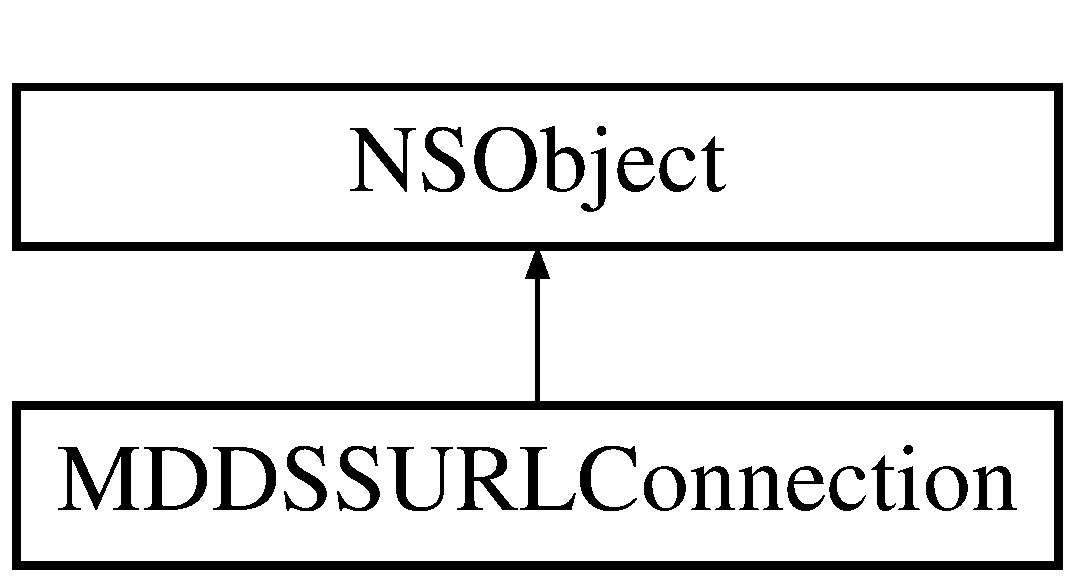
\includegraphics[height=2.000000cm]{interface_m_d_d_s_s_u_r_l_connection}
\end{center}
\end{figure}
\subsection*{Class Methods}
\begin{DoxyCompactItemize}
\item 
(instancetype) + \hyperlink{interface_m_d_d_s_s_u_r_l_connection_a4adceb5901feaca4d9f185830628c552}{json\-Connection\-To\-Host\-With\-Port\-:path\-:params\-:completion\-Handler\-:}
\end{DoxyCompactItemize}


\subsection{Detailed Description}
\hyperlink{interface_m_d_d_s_s_u_r_l_connection}{M\-D\-D\-S\-S\-U\-R\-L\-Connection} class. Inet connection layer. 

\subsection{Method Documentation}
\hypertarget{interface_m_d_d_s_s_u_r_l_connection_a4adceb5901feaca4d9f185830628c552}{\index{M\-D\-D\-S\-S\-U\-R\-L\-Connection@{M\-D\-D\-S\-S\-U\-R\-L\-Connection}!json\-Connection\-To\-Host\-With\-Port\-:path\-:params\-:completion\-Handler\-:@{json\-Connection\-To\-Host\-With\-Port\-:path\-:params\-:completion\-Handler\-:}}
\index{json\-Connection\-To\-Host\-With\-Port\-:path\-:params\-:completion\-Handler\-:@{json\-Connection\-To\-Host\-With\-Port\-:path\-:params\-:completion\-Handler\-:}!MDDSSURLConnection@{M\-D\-D\-S\-S\-U\-R\-L\-Connection}}
\subsubsection[{json\-Connection\-To\-Host\-With\-Port\-:path\-:params\-:completion\-Handler\-:}]{\setlength{\rightskip}{0pt plus 5cm}+ (instancetype) json\-Connection\-To\-Host\-With\-Port\-: 
\begin{DoxyParamCaption}
\item[{(N\-S\-String $\ast$)}]{host\-And\-Port}
\item[{path:(N\-S\-String $\ast$)}]{path}
\item[{params:(N\-S\-Dictionary $\ast$)}]{params}
\item[{completionHandler:(void($^\wedge$)(N\-S\-Dictionary $\ast$, N\-S\-Error $\ast$))}]{handler}
\end{DoxyParamCaption}
}}\label{interface_m_d_d_s_s_u_r_l_connection_a4adceb5901feaca4d9f185830628c552}
Create a instance of \hyperlink{interface_m_d_d_s_s_u_r_l_connection}{M\-D\-D\-S\-S\-U\-R\-L\-Connection}, calls the d\-S\-S (async) and parses the json response. The result will be passed to the completion\-Handler (block) 

The documentation for this class was generated from the following file\-:\begin{DoxyCompactItemize}
\item 
D\-S\-Menu/\-M\-D\-D\-S\-S\-Manager/M\-D\-D\-S\-S\-U\-R\-L\-Connection.\-h\end{DoxyCompactItemize}

\hypertarget{interface_m_d_main_preferences_view_controller}{\section{M\-D\-Main\-Preferences\-View\-Controller Class Reference}
\label{interface_m_d_main_preferences_view_controller}\index{M\-D\-Main\-Preferences\-View\-Controller@{M\-D\-Main\-Preferences\-View\-Controller}}
}
Inheritance diagram for M\-D\-Main\-Preferences\-View\-Controller\-:\begin{figure}[H]
\begin{center}
\leavevmode
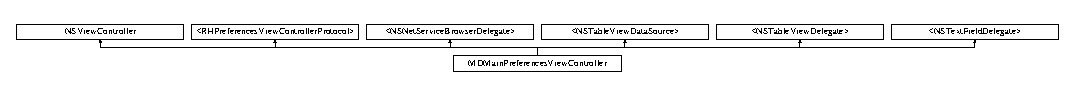
\includegraphics[height=0.740741cm]{interface_m_d_main_preferences_view_controller}
\end{center}
\end{figure}
\subsection*{Properties}
\begin{DoxyCompactItemize}
\item 
\hypertarget{interface_m_d_main_preferences_view_controller_aa61a9ae962dc2a8d7fd5be8f36c8cf62}{I\-B\-Outlet N\-S\-Table\-View $\ast$ {\bfseries table\-View}}\label{interface_m_d_main_preferences_view_controller_aa61a9ae962dc2a8d7fd5be8f36c8cf62}

\item 
\hypertarget{interface_m_d_main_preferences_view_controller_a9dfae1433203c8ec852648b2da348020}{I\-B\-Outlet N\-S\-Text\-Field $\ast$ {\bfseries address\-Text\-Field}}\label{interface_m_d_main_preferences_view_controller_a9dfae1433203c8ec852648b2da348020}

\item 
\hypertarget{interface_m_d_main_preferences_view_controller_a6f4d01ff12f22736a888a23bd51ad22f}{I\-B\-Outlet N\-S\-Text\-Field $\ast$ {\bfseries title\-Text\-Field}}\label{interface_m_d_main_preferences_view_controller_a6f4d01ff12f22736a888a23bd51ad22f}

\item 
\hypertarget{interface_m_d_main_preferences_view_controller_a44cd3a513344639ec3e1e7e6bc8aed99}{I\-B\-Outlet N\-S\-Text\-Field $\ast$ {\bfseries server\-Address\-Label}}\label{interface_m_d_main_preferences_view_controller_a44cd3a513344639ec3e1e7e6bc8aed99}

\item 
\hypertarget{interface_m_d_main_preferences_view_controller_a598365193d39fd6737dfb0e73a5a01c5}{I\-B\-Outlet N\-S\-Text\-Field $\ast$ {\bfseries token\-Label}}\label{interface_m_d_main_preferences_view_controller_a598365193d39fd6737dfb0e73a5a01c5}

\item 
\hypertarget{interface_m_d_main_preferences_view_controller_a7a49586da4593f1a245e506a493bf1c5}{I\-B\-Outlet N\-S\-Text\-Field $\ast$ {\bfseries token\-Field}}\label{interface_m_d_main_preferences_view_controller_a7a49586da4593f1a245e506a493bf1c5}

\end{DoxyCompactItemize}


The documentation for this class was generated from the following file\-:\begin{DoxyCompactItemize}
\item 
mac\-D\-S/\-Preferences/M\-D\-Main\-Preferences\-View\-Controller.\-h\end{DoxyCompactItemize}

\hypertarget{interface_m_d_scene_menu_item}{\section{M\-D\-Scene\-Menu\-Item Class Reference}
\label{interface_m_d_scene_menu_item}\index{M\-D\-Scene\-Menu\-Item@{M\-D\-Scene\-Menu\-Item}}
}


{\ttfamily \#import $<$M\-D\-Scene\-Menu\-Item.\-h$>$}

Inheritance diagram for M\-D\-Scene\-Menu\-Item\-:\begin{figure}[H]
\begin{center}
\leavevmode
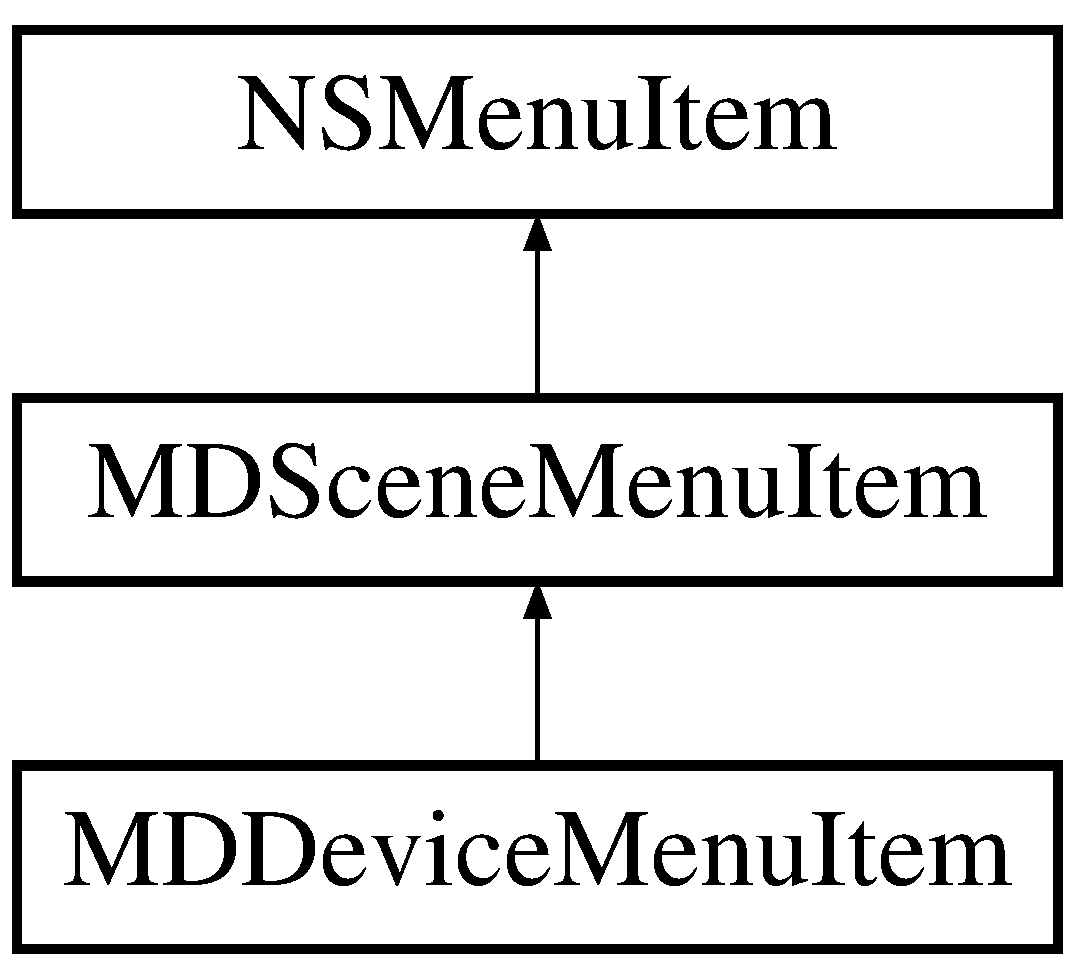
\includegraphics[height=3.000000cm]{interface_m_d_scene_menu_item}
\end{center}
\end{figure}
\subsection*{Properties}
\begin{DoxyCompactItemize}
\item 
N\-S\-Integer \hyperlink{interface_m_d_scene_menu_item_aa65f24d6bf8e466abdb0d32ee07b3c44}{group}
\end{DoxyCompactItemize}


\subsection{Detailed Description}
M\-D\-Zone\-Menu\-Item\-Click\-Type. Class for Scene Menu Item 

\subsection{Property Documentation}
\hypertarget{interface_m_d_scene_menu_item_aa65f24d6bf8e466abdb0d32ee07b3c44}{\index{M\-D\-Scene\-Menu\-Item@{M\-D\-Scene\-Menu\-Item}!group@{group}}
\index{group@{group}!MDSceneMenuItem@{M\-D\-Scene\-Menu\-Item}}
\subsubsection[{group}]{\setlength{\rightskip}{0pt plus 5cm}-\/ (N\-S\-Integer) group\hspace{0.3cm}{\ttfamily [read]}, {\ttfamily [write]}, {\ttfamily [atomic]}, {\ttfamily [assign]}}}\label{interface_m_d_scene_menu_item_aa65f24d6bf8e466abdb0d32ee07b3c44}
group Number (ex. 1 = yellow) which will be used for further actions 

The documentation for this class was generated from the following file\-:\begin{DoxyCompactItemize}
\item 
D\-S\-Menu/\-Menu/M\-D\-Scene\-Menu\-Item.\-h\end{DoxyCompactItemize}

\hypertarget{interface_m_d_zone_menu_item}{\section{M\-D\-Zone\-Menu\-Item Class Reference}
\label{interface_m_d_zone_menu_item}\index{M\-D\-Zone\-Menu\-Item@{M\-D\-Zone\-Menu\-Item}}
}


{\ttfamily \#import $<$M\-D\-Zone\-Menu\-Item.\-h$>$}

Inheritance diagram for M\-D\-Zone\-Menu\-Item\-:\begin{figure}[H]
\begin{center}
\leavevmode
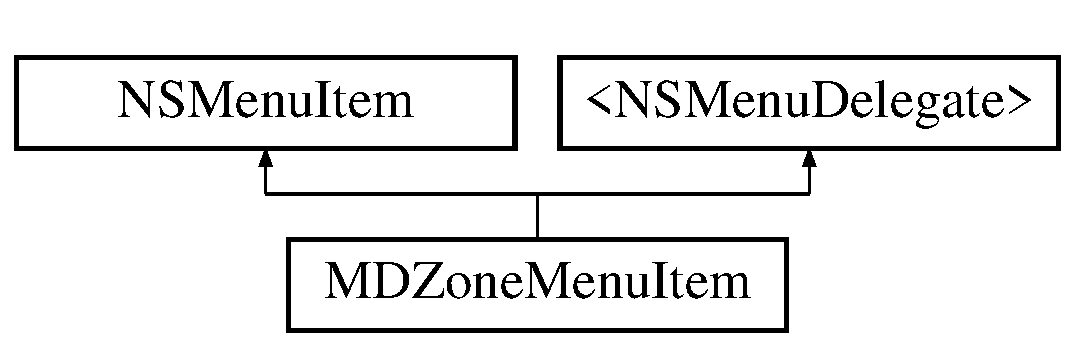
\includegraphics[height=2.000000cm]{interface_m_d_zone_menu_item}
\end{center}
\end{figure}
\subsection*{Class Methods}
\begin{DoxyCompactItemize}
\item 
\hypertarget{interface_m_d_zone_menu_item_aee59d24738e6900cf6d5cd545af9eda2}{(\hyperlink{interface_m_d_zone_menu_item}{M\-D\-Zone\-Menu\-Item} $\ast$) + {\bfseries menu\-Item\-With\-Zone\-Dictionary\-:}}\label{interface_m_d_zone_menu_item_aee59d24738e6900cf6d5cd545af9eda2}

\end{DoxyCompactItemize}
\subsection*{Properties}
\begin{DoxyCompactItemize}
\item 
N\-S\-String $\ast$ \hyperlink{interface_m_d_zone_menu_item_a0233a890891b84a2c30226439a3185ea}{zone\-Id}
\item 
\hyperlink{interface_m_d_scene_menu_item}{M\-D\-Scene\-Menu\-Item} $\ast$ \hyperlink{interface_m_d_zone_menu_item_a6a4957a6b3fe720a65aa67f6c07be18f}{clicked\-Submenu}
\item 
\hypertarget{interface_m_d_zone_menu_item_a17353c5d03094c9e62a49e1127854eb9}{M\-D\-Zone\-Menu\-Item\-Click\-Type {\bfseries click\-Type}}\label{interface_m_d_zone_menu_item_a17353c5d03094c9e62a49e1127854eb9}

\end{DoxyCompactItemize}


\subsection{Detailed Description}
M\-D\-Zone\-Menu\-Item\-Click\-Type. This class represents a Zone as a Menu\-Item. 

\subsection{Property Documentation}
\hypertarget{interface_m_d_zone_menu_item_a6a4957a6b3fe720a65aa67f6c07be18f}{\index{M\-D\-Zone\-Menu\-Item@{M\-D\-Zone\-Menu\-Item}!clicked\-Submenu@{clicked\-Submenu}}
\index{clicked\-Submenu@{clicked\-Submenu}!MDZoneMenuItem@{M\-D\-Zone\-Menu\-Item}}
\subsubsection[{clicked\-Submenu}]{\setlength{\rightskip}{0pt plus 5cm}-\/ ({\bf M\-D\-Scene\-Menu\-Item}$\ast$) clicked\-Submenu\hspace{0.3cm}{\ttfamily [read]}, {\ttfamily [write]}, {\ttfamily [atomic]}, {\ttfamily [strong]}}}\label{interface_m_d_zone_menu_item_a6a4957a6b3fe720a65aa67f6c07be18f}
if a submenu was clicked, this ivar will be filled. \hypertarget{interface_m_d_zone_menu_item_a0233a890891b84a2c30226439a3185ea}{\index{M\-D\-Zone\-Menu\-Item@{M\-D\-Zone\-Menu\-Item}!zone\-Id@{zone\-Id}}
\index{zone\-Id@{zone\-Id}!MDZoneMenuItem@{M\-D\-Zone\-Menu\-Item}}
\subsubsection[{zone\-Id}]{\setlength{\rightskip}{0pt plus 5cm}-\/ (N\-S\-String$\ast$) zone\-Id\hspace{0.3cm}{\ttfamily [read]}, {\ttfamily [write]}, {\ttfamily [atomic]}, {\ttfamily [strong]}}}\label{interface_m_d_zone_menu_item_a0233a890891b84a2c30226439a3185ea}
the connected zone\-Id 

The documentation for this class was generated from the following file\-:\begin{DoxyCompactItemize}
\item 
mac\-D\-S/\-Menu/M\-D\-Zone\-Menu\-Item.\-h\end{DoxyCompactItemize}

%--- End generated contents ---

% Index
\newpage
\phantomsection
\addcontentsline{toc}{chapter}{Index}
\printindex

\end{document}
